% Options for packages loaded elsewhere
\PassOptionsToPackage{unicode}{hyperref}
\PassOptionsToPackage{hyphens}{url}
\PassOptionsToPackage{dvipsnames,svgnames*,x11names*}{xcolor}
%
\documentclass[12pt,
  landscape]{article}
\usepackage{lmodern}
\usepackage{amsmath}
\usepackage{ifxetex,ifluatex}
\ifnum 0\ifxetex 1\fi\ifluatex 1\fi=0 % if pdftex
  \usepackage[T1]{fontenc}
  \usepackage[utf8]{inputenc}
  \usepackage{textcomp} % provide euro and other symbols
  \usepackage{amssymb}
\else % if luatex or xetex
  \usepackage{unicode-math}
  \defaultfontfeatures{Scale=MatchLowercase}
  \defaultfontfeatures[\rmfamily]{Ligatures=TeX,Scale=1}
\setmainfont{IBM Plex Sans}
\setsansfont{Patua One}
\fi
% Use upquote if available, for straight quotes in verbatim environments
\IfFileExists{upquote.sty}{\usepackage{upquote}}{}
\IfFileExists{microtype.sty}{% use microtype if available
  \usepackage[]{microtype}
  \UseMicrotypeSet[protrusion]{basicmath} % disable protrusion for tt fonts
}{}
\makeatletter
\@ifundefined{KOMAClassName}{% if non-KOMA class
  \IfFileExists{parskip.sty}{%
    \usepackage{parskip}
  }{% else
    \setlength{\parindent}{0pt}
    \setlength{\parskip}{6pt plus 2pt minus 1pt}}
}{% if KOMA class
  \KOMAoptions{parskip=half}}
\makeatother
\usepackage[dvipsnames]{xcolor}
\IfFileExists{xurl.sty}{\usepackage{xurl}}{} % add URL line breaks if available
\IfFileExists{bookmark.sty}{\usepackage{bookmark}}{\usepackage{hyperref}}
\hypersetup{
  pdftitle={Reading Group 20/03/2024},
  colorlinks=true,
  linkcolor=blue,
  filecolor=Maroon,
  citecolor=Blue,
  urlcolor=Blue,
  pdfcreator={LaTeX via pandoc}}
\urlstyle{same} % disable monospaced font for URLs
\usepackage[a4paper, margin=1in]{geometry}

\usepackage{longtable,booktabs}
\usepackage{calc} % for calculating minipage widths
% Correct order of tables after \paragraph or \subparagraph
\usepackage{etoolbox}
\makeatletter
\patchcmd\longtable{\par}{\if@noskipsec\mbox{}\fi\par}{}{}
\makeatother
% Allow footnotes in longtable head/foot
\IfFileExists{footnotehyper.sty}{\usepackage{footnotehyper}}{\usepackage{footnote}}
\makesavenoteenv{longtable}
\usepackage{graphicx}
\makeatletter
\def\maxwidth{\ifdim\Gin@nat@width>\linewidth\linewidth\else\Gin@nat@width\fi}
\def\maxheight{\ifdim\Gin@nat@height>\textheight\textheight\else\Gin@nat@height\fi}
\makeatother
% Scale images if necessary, so that they will not overflow the page
% margins by default, and it is still possible to overwrite the defaults
% using explicit options in \includegraphics[width, height, ...]{}
\setkeys{Gin}{width=\maxwidth,height=\maxheight,keepaspectratio}
% Set default figure placement to htbp
\makeatletter
\def\fps@figure{htbp}
\makeatother
\setlength{\emergencystretch}{3em} % prevent overfull lines
\providecommand{\tightlist}{%
  \setlength{\itemsep}{0pt}\setlength{\parskip}{0pt}}
\setcounter{secnumdepth}{-\maxdimen} % remove section numbering
% Make \paragraph and \subparagraph free-standing
\ifx\paragraph\undefined\else
  \let\oldparagraph\paragraph
  \renewcommand{\paragraph}[1]{\oldparagraph{#1}\mbox{}}
\fi
\ifx\subparagraph\undefined\else
  \let\oldsubparagraph\subparagraph
  \renewcommand{\subparagraph}[1]{\oldsubparagraph{#1}\mbox{}}
\fi
\pagestyle{empty}
\makeatletter
\@ifpackageloaded{caption}{}{\usepackage{caption}}
\AtBeginDocument{%
\ifdefined\contentsname
  \renewcommand*\contentsname{Table of contents}
\else
  \newcommand\contentsname{Table of contents}
\fi
\ifdefined\listfigurename
  \renewcommand*\listfigurename{List of Figures}
\else
  \newcommand\listfigurename{List of Figures}
\fi
\ifdefined\listtablename
  \renewcommand*\listtablename{List of Tables}
\else
  \newcommand\listtablename{List of Tables}
\fi
\ifdefined\figurename
  \renewcommand*\figurename{Figure}
\else
  \newcommand\figurename{Figure}
\fi
\ifdefined\tablename
  \renewcommand*\tablename{Table}
\else
  \newcommand\tablename{Table}
\fi
}
\@ifpackageloaded{float}{}{\usepackage{float}}
\floatstyle{ruled}
\@ifundefined{c@chapter}{\newfloat{codelisting}{h}{lop}}{\newfloat{codelisting}{h}{lop}[chapter]}
\floatname{codelisting}{Listing}
\newcommand*\listoflistings{\listof{codelisting}{List of Listings}}
\makeatother
\makeatletter
\makeatother
\makeatletter
\@ifpackageloaded{caption}{}{\usepackage{caption}}
\@ifpackageloaded{subcaption}{}{\usepackage{subcaption}}
\makeatother
\ifluatex
  \usepackage{selnolig}  % disable illegal ligatures
\fi

\title{\textbf{Reading Group 20/03/2024}}
\usepackage{etoolbox}
\makeatletter
\providecommand{\subtitle}[1]{% add subtitle to \maketitle
  \apptocmd{\@title}{\par {\large #1 \par}}{}{}
}
\makeatother
\subtitle{Md Musfiqur Rahman, Murat Kocaoglu (2024): Modular Learning of
Deep Causal Generative Models for High-dimensional Causal Inference}
\author{}
\date{}

% my preamble additions =============================================================

% left justify text with ragged right edge =====================================
\usepackage[document]{ragged2e}

% page numbering ===============================================================
\usepackage{fancyhdr}
\pagestyle{fancy}
\fancyhf{}
\renewcommand{\headrulewidth}{0pt}
\fancyfoot[C]{\footnotesize\textcolor{gray}{Reading Group 20/03/2024}}
\fancyfoot[R]{\footnotesize\textcolor{gray}{\thepage}}

% change default spacing before each new paragraph (sets as text height) =======
\setlength\parskip{1em plus 0.1em minus 0.2em}

% set formatting for section and subsection headings ===========================
% adding a period after section numbering
% \usepackage{titlesec}
% \titlelabel{\thetitle.\quad}
% comment/uncomment the next line to insert a page break before each new H1
\let\oldsection\section
\renewcommand\section{\clearpage\oldsection}

% changing options for table/figure captions ===================================
% uncomment the below lines to just number figures/tables sequentially
% throughout entire document
% \renewcommand{\thetable}{\thesection.\arabic{table}}
% \renewcommand{\thefigure}{\thesection.\arabic{figure}}

\usepackage[labelfont=it,textfont=it,singlelinecheck=off,justification=raggedright,labelsep=period]{caption}

% resets table/figure counters within each section/subsection ==================
% \usepackage{chngcntr}
% \counterwithin*{table}{section}
%\counterwithin*{table}{subsection}
% \counterwithin*{figure}{section}
%\counterwithin*{figure}{subsection}

\usepackage[breakable]{tcolorbox}

\definecolor{cosmiclatte}{RGB}{255, 248, 231}
\definecolor{justoffwhite}{RGB}{255, 254, 250}

%\definecolor{notes-bg}{RGB}{254, 250, 233}
%\definecolor{notes-frame}{RGB}{222, 217, 193}

%\definecolor{Questions-bg}{RGB}{236, 239, 244}
%\definecolor{Questions-frame}{RGB}{236, 239, 244}

\definecolor{notes-bg}{RGB}{244, 247, 252}
\definecolor{notes-frame}{RGB}{233, 235, 238}
\definecolor{notes-text}{RGB}{47, 54, 61}

\definecolor{slide-titles}{RGB}{220, 50, 47}

\usepackage{pagecolor}
\usepackage{afterpage}

\renewcommand{\baselinestretch}{1.5}

% resize headings =============================

\makeatletter

\renewcommand{\section}{\@startsection
{section}%                   % the name
{1}%                         % the level
{\z@}%                       % the indent / 0mm
{3\baselineskip}%            % the before skip / -3.5ex \@plus -1ex \@minus -.2ex
{3\baselineskip}%          % the after skip / 2.3ex \@plus .2ex
{\sffamily\huge\bfseries}} % the style

\renewcommand{\subsection}{\@startsection
{subsection}%                   % the name
{2}%                         % the level
{\z@}%                       % the indent / 0mm
{3\baselineskip}%            % the before skip / -3.5ex \@plus -1ex \@minus -.2ex
{.75\baselineskip}%          % the after skip / 2.3ex \@plus .2ex
{\sffamily\Large\bfseries\textcolor{slide-titles}}} % the style

\renewcommand{\subsubsection}{\@startsection
{subsubsection}%                   % the name
{3}%                         % the level
{\z@}%                       % the indent / 0mm
{3\baselineskip}%            % the before skip / -3.5ex \@plus -1ex \@minus -.2ex
{.75\baselineskip}%          % the after skip / 2.3ex \@plus .2ex
{\large\bfseries}} % the style

\makeatother

\usepackage[export]{adjustbox}

% ===================================================================================

\begin{document}


      % \maketitle
    \begin{center}
    \vspace*{5cm}
    {\Huge\bfseries Reading Group 20/03/2024}\\
        \end{center}  
    % turn off page numbering for titlepage
    \thispagestyle{empty}
        \newpage
  





\newpage

\vspace*{2.5cm}

\begin{center}

\section{Introduction}\label{introduction}

\end{center}

\newpage

\subsection{Background - Structural Causal
Model}\label{background---structural-causal-model}

\begin{itemize}
\tightlist
\item
  An SCM \(\mathcal{M}\) is a \(5\)-tuple
  \(\mathcal{M}=(\mathcal{V}, \mathcal{N}, \mathcal{U}, \mathcal{F}, P(.) )\),
\item
  Each observed variable \(V_i\in\mathcal{V}\) is realized as an
  evaluation of the function \(f_i\in\mathcal{F}\) looks at a subset of
  the remaining observed variables

  \begin{itemize}
  \tightlist
  \item
    Remaining observed variables \(Pa_i\subset \mathcal{V}\) (Parent Set
    of \(V_i\))
  \item
    Unobserved exogenous noise variable \(E_i\in \mathcal{N}\)
  \item
    Unobserved confounding variable \(U_i\in\mathcal{U}\)
  \end{itemize}
\item
  \(P(.)\) is a product joint distribution over all unobserved variables
  \(\mathcal{N}\cup\mathcal{U}\)
\end{itemize}

\newpage

\subsection{Background - SCMs and Causal
Graphs}\label{background---scms-and-causal-graphs}

\begin{itemize}
\tightlist
\item
  Each SCM induces a directed graph called the causal graph or acyclic
  directed mixed graph (ADMG)
\item
  In the context of this paper, the graph is still acyclic, but no
  longer a DAG

  \begin{itemize}
  \tightlist
  \item
    The graph can handle bidirectional edges
    (e.g.~\(V_i \leftrightarrow V_j\)) to represent unobserved
    confounders
  \end{itemize}
\item
  \(V_i\) is called an ancestor of \(V_j\) if there is a directed path
  from \(V_i\) to \(V_j\)
\item
  A subset \(g \subset G\) is called a c-component if it is a maximal
  set of nodes in \(G\) that are connected by bi-directed paths
\end{itemize}

\newpage

\subsection{Introduction}\label{introduction-1}

\begin{itemize}
\tightlist
\item
  Goal: Perform Causal Inference, e.g.~evaluating the causal effect of
  an intervention on a system of interest
\item
  Today, most of our datasets contain high-dimensional variables, such
  as images
\item
  Modern deep learning architectures can handle high dimensional data
  and solve ML problems such as prediction or learning distributions
\item
  However, they are not designed to perform causal inference

  \begin{itemize}
  \tightlist
  \item
    They fail to generalize where there exists spurious correlations in
    the data
  \end{itemize}
\end{itemize}

\newpage

\subsection{Main Example of the paper}\label{main-example-of-the-paper}

\begin{itemize}
\tightlist
\item
  Healthcare dataset with Symptoms, Diagnosis and XrayImages of a
  collection of patients

  \begin{itemize}
  \tightlist
  \item
    Contains a mixture data from two hospitals in different cities where
    one of the cities is more wealthy, where patients are less likely to
    fall sick on average
  \end{itemize}
\item
  Hospital location acts as a latent confounder that affect both the
  Symptoms and Diagnosis
\end{itemize}

\newpage

\subsection{Main Example of the
paper}\label{main-example-of-the-paper-1}

\begin{figure}
\centering
\includegraphics[max height=0.5\paperheight]{imgs/main\_example.PNG}
\caption{Causal Graph of the main example}
\end{figure}

\newpage

\subsection{Main Idea of the paper}\label{main-idea-of-the-paper}

\begin{itemize}
\tightlist
\item
  The paper proposes a modular sampling-based framework for deep causal
  generative models

  \begin{itemize}
  \tightlist
  \item
    Collect observational samples and use these samples to estimate the
    interventional distribution
  \end{itemize}
\item
  In this paper, \(\mathcal{L}_1\), \(\mathcal{L}_2\), and
  \(\mathcal{L}_3\) distributions as notation for observational,
  interventional, and counterfactual distributions respectively
\item
  Using deep learning architectures that mimic the causal structure of
  the system
\item
  Using pre-trained generative models like DALL-E, ChatGPT or Bard
\end{itemize}

\newpage

\subsection{Main Idea of the paper}\label{main-idea-of-the-paper-1}

\begin{figure}
\centering
\includegraphics[max height=0.5\paperheight]{imgs/main\_arch.PNG}
\caption{Deep Causal Generative Model}
\end{figure}

\newpage

\vspace*{2.5cm}

\begin{center}

\section{Deep Causal Generative Models with Unobserved
Confounders}\label{deep-causal-generative-models-with-unobserved-confounders}

\end{center}

\newpage

\subsection{Definition}\label{definition}

Let a SCM \(\mathcal{M}\) be made up of functions
\(X_i = f_i(Pa_i, E_i)\).

A neural net architecture \(\mathbb{G}\) is called a deep causal
generative model (DCM) for an ADMG \(G\) inducing a distribution \(Q\)
if it is composed of a collection of neural nets, one \(\mathbb{G}_i\)
for each \(V_i\in\mathcal{V}\) such that

\begin{itemize}
\tightlist
\item
  Each \(\mathbb{G}_i\) accepts a sufficiently high-dimensional noise
  vector \(N_i\)
\item
  The output of \(\mathbb{G}_j\) is input to
  \(\mathbb{G}_i \Leftrightarrow V_j\in Pa_G(V_i)\)
\item
  \(N_i=N_j \Leftrightarrow V_i\leftrightarrow V_j\)
\end{itemize}

Note that \(\mathbb{G}\) will contain \textbf{one neural net per
observed variable}:
\(\mathbb{G}=\{\mathbb{G}_{Z_1},\mathbb{G}_{Z_2}, ... \}\)

\newpage

\subsection{Intuition}\label{intuition}

\begin{itemize}
\tightlist
\item
  Let \(D\sim P(\mathcal{V})\) be an observational sample
\item
  Train a DCM \(\mathbb{G}\) that fits the observational distribution
  \(P(\mathcal{V})\) to sample the interventional distribution
  \(\mathcal{L}_2\)
\item
  Training involves identifying which causal mechanisms should be
  trained together based on their dependencies in the causal graph
\item
  Start with the first neural network
  \(\mathbb{G}_{Z_1} \in \mathbb{G}\) to learn a mapping to sample
  \(P(Z_1 | Z_3, X_1)\)
\item
  The training preserve the integrity of c-components and factorize the
  joint distribution of them to yield \(P(\mathcal{V})\)
\end{itemize}

\Leftarrow

\begin{figure}
\centering
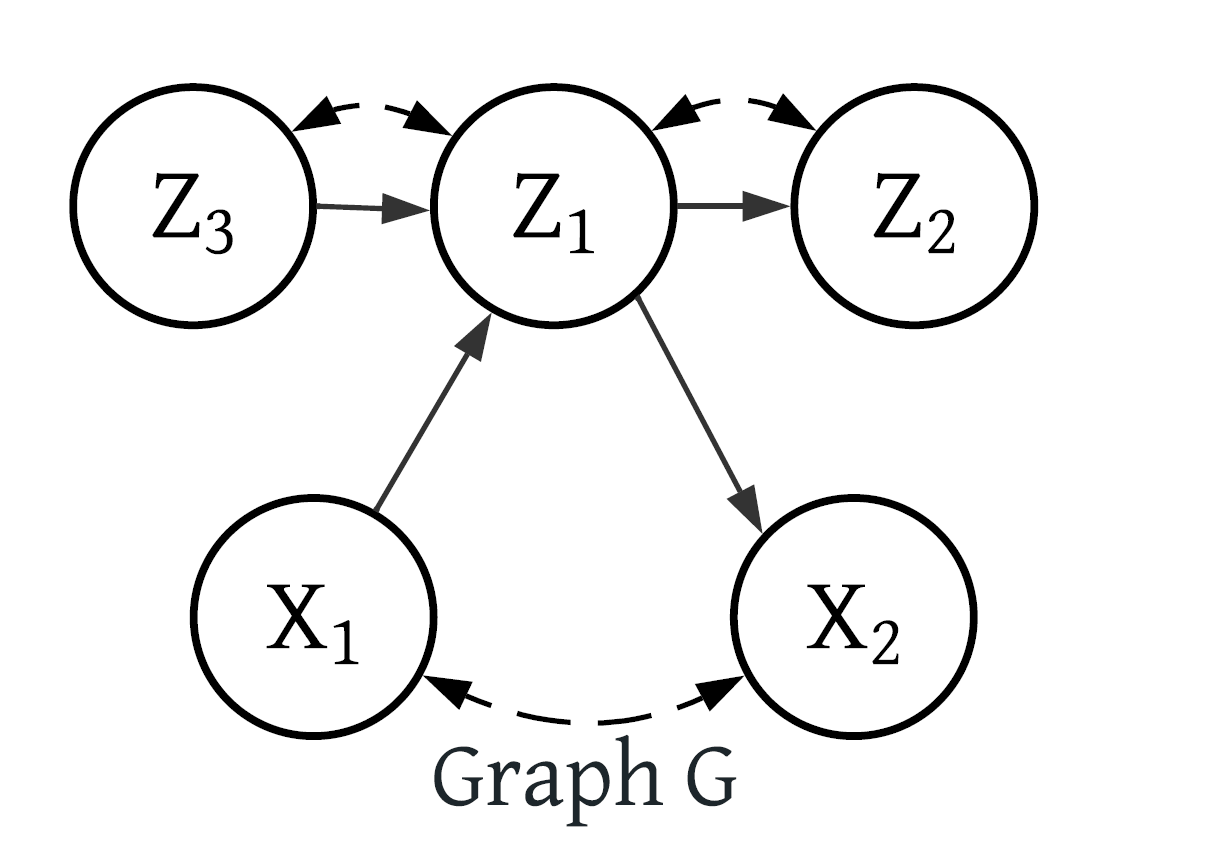
\includegraphics[max height=0.5\paperheight]{imgs/CG.PNG}
\caption{Example Causal Graph: \(X\) denotes the first c-component,
\(Z\) the second c-component}
\end{figure}

\newpage

\subsection{Intuition}\label{intuition-1}

\begin{figure}
\centering
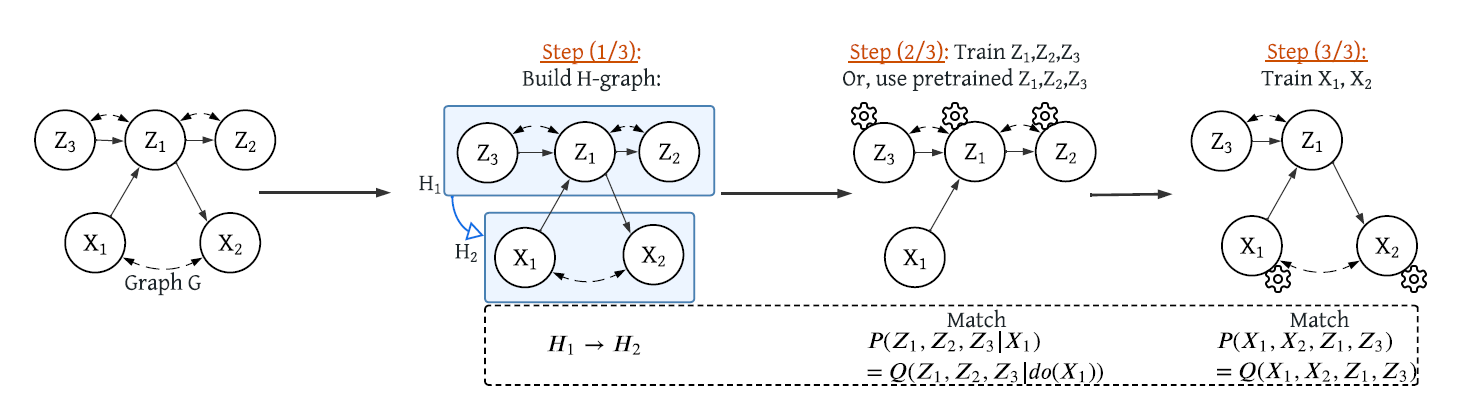
\includegraphics[max height=0.5\paperheight]{imgs/DCM.PNG}
\caption{Modular training in 3 steps. Step 1: Since
\(P(X_1,X_2| do(Z_1)) \neq P(X_1,X_2| Z_1)\), add an edge from
c-component \(H_1: [Z_1,Z_2,Z_3]\) to c-component \(H_2: [X_1,X_2]\).
Step 2: Train only the mechanisms in \(H_1\) to match
\(P(Z_1,Z_2,Z_3|X_1) = Q(Z_1,Z_2,Z_3|do(X_1))\). Step 3: Train only
\(H_2\) while using pre-trained \(Z_1,Z_3\) to match
\(P(X_1,X_2,Z_1, Z_3) = Q(X_1,X_2,Z_1, Z_3)\)}
\end{figure}

\newpage

\subsection{Intuition}\label{intuition-2}

\begin{itemize}
\tightlist
\item
  By training mechanisms in the same c-component together, the
  complexity of matching joint distributions involving high and
  low-dimensional variables is significantly reduced.
\item
  Modularizing the training process allows for more efficient training
  and simplifies the overall learning task.
\end{itemize}

\newpage

\subsection{Algorithm}\label{algorithm}

\begin{algorithm}[H]
\small
    \caption{Construct\_Hgraph($G$)}
\begin{algorithmic}[1]
 \STATE {\bfseries Input:} Causal Graph $G$
 % \FOR{{\bfseries each} $I \in \mathcal{I}$}
\STATE $\mathcal{C} \leftarrow \mathrm{get\_ccomponents}(G)$
\STATE Create nodes $H_k=C_k$ in $\mathcal{H}$, $\forall C_k \in \mathcal{C} $
% \ENDFOR
% \FOR{{\bfseries each} $I \in \mathcal{I}$}
\FOR{{\bfseries each} $H_s,H_t \in \mathcal{H}$ such that $s\neq t$}
% \IF{ $\exists (V_s,V_t) \in (H_s, H_t)$ such that $V_s = Pa(V_t)$ and
% $P(H_t|\doo(V_s)) \neq P(H_t|V_s)$\label{alg2:do-calculus-check}
% } 
\IF{$P(H_t|\doo(pa(H_t) \cap H_s))$ \\
$\neq P(H_t|pa(H_t) \cap H_s)$}
\label{alg2:do-calculus-check}
\STATE $\mathcal{H}.add(H_s \rightarrow H_t)$
\ENDIF
\ENDFOR
\STATE $\mathcal{H} \leftarrow$  $\mathrm{Merge}$($\mathcal{H}$, $cyc$), $\forall cyc \in Cycles(\mathcal{H})$
\label{alg:h-graph-mergecycles}
\STATE {\bfseries Return:} $\mathcal{H}$
\end{algorithmic}
\label{construct-H-graph}
\end{algorithm}

\end{document}
